\documentclass[12pt,a4paper]{ctexart}

% ============ 页边距 ============
\usepackage[top=2.5cm, bottom=2.5cm, left=2.5cm, right=2.5cm]{geometry}

% ============ 中文支持 ============
\usepackage{xeCJK}

% ============ 数学公式 ============
\usepackage{amsmath, amssymb}

% ============ 图表 ============
\usepackage{graphicx}
\usepackage{float}
\usepackage{subcaption}
\usepackage{booktabs}
\usepackage{array}
\usepackage{multirow}

% ============ 超链接 ============
\usepackage[colorlinks=true, linkcolor=blue, citecolor=blue, urlcolor=blue]{hyperref}

% ============ 代码高亮 ============
\usepackage{listings}
\usepackage{xcolor}
\lstset{
    basicstyle=\ttfamily\small,
    numbers=left,
    numberstyle=\tiny\gray,
    frame=single,
    breaklines=true,
    showstringspaces=false,
    tabsize=2,
    keywordstyle=\color{blue},
    commentstyle=\color{gray},
    stringstyle=\color{red},
}

% ============ 标题格式 ============
\usepackage{titlesec}
\titleformat{\section}{\large\bfseries}{\thesection}{1em}{}
\titleformat{\subsection}{\normalsize\bfseries}{\thesubsection}{1em}{}

\begin{document}

% ============ 封面 ============
\begin{center}
    {\LARGE \textbf{任务1实验报告}}\\[0.5cm]
    {\Large \textbf{基于强化学习的倒立摆控制}}\\[1.5cm]
    {\large 课程：AI赋能自动控制原理}\\[0.3cm]
    {\large 日期：2025年7月}\\[1cm]
    \rule{\textwidth}{0.5pt}
\end{center}

\vspace{1cm}

% ============ 1 问题分析 ============
\section{问题分析}

\subsection{Cart Pole系统与强化学习环境}

\subsubsection{状态空间与动作空间}

Cart Pole（小车-倒立摆）是自动控制原理中的经典非线性系统控制案例。系统由一辆可在水平轨道上左右移动的小车和一根铰接在小车上的摆杆组成。控制目标是通过对小车施加水平力，使摆杆始终保持直立状态，不会因重力倒下。该问题具有重要的教学意义：它帮助学生理解非线性系统的动态特性与控制难度，直观认识强化学习在解决复杂控制任务中的优势。

本实验使用OpenAI Gymnasium提供的CartPole-v1环境。系统的状态空间为4维连续向量，各状态量的物理含义如表\ref{tab:state_space}所示。

\begin{table}[H]
\centering
\caption{CartPole-v1状态空间定义}
\label{tab:state_space}
\begin{tabular}{cclcc}
\toprule
\textbf{序号} & \textbf{符号} & \textbf{含义} & \textbf{单位} & \textbf{理论范围} \\
\midrule
0 & \(x\) & 小车在轨道上的位置 & m & \([-4.8, 4.8]\) \\
1 & \(\dot{x}\) & 小车的水平速度 & m/s & 未限制 \\
2 & \(\theta\) & 摆杆与垂直方向的夹角 & rad & \([-0.4189, 0.4189]\) \\
3 & \(\dot{\theta}\) & 摆杆的角速度 & rad/s & 未限制 \\
\bottomrule
\end{tabular}
\end{table}

动作空间为离散二值动作：动作0表示对小车施加向左的推力（使小车左移），动作1表示对小车施加向右的推力（使小车右移）。环境的终止条件包括：(1) 摆杆角度\(|\theta|>12^{\circ}\)（0.2094\,rad）；(2) 小车位置\(|x|>2.4\)\,m（相对于中心）；(3) 回合步数达到500步（v1版本）。每步存活可获得+1奖励，单回合最高奖励为500。随机策略在此环境下的平均奖励仅为21步，远低于满分500，说明该任务需要通过强化学习来掌握合理的控制策略。

\subsection{算法与奖励函数设计}

\subsubsection{算法选择及基本原理}

为全面评估不同强化学习范式在连续状态控制任务中的表现，本实验选用两种具有代表性的深度强化学习算法：基于值函数的DQN（Deep Q-Network）和基于策略梯度的PPO（Proximal Policy Optimization）。

\textbf{(1) DQN算法}

DQN是基于值函数的深度强化学习算法，核心思想是使用深度神经网络近似最优动作价值函数\(Q^*(s,a)\)，通过最小化时序差分（Temporal Difference, TD）误差来迭代更新网络参数。其损失函数定义为：

\begin{equation}
L(\theta) = \mathbb{E}_{(s,a,r,s')\sim\mathcal{D}}\left[\left(r + \gamma \max_{a'} Q(s', a'; \theta^-) - Q(s, a; \theta)\right)^2\right]
\end{equation}

其中\(\theta\)为在线网络的参数，\(\theta^-\)为目标网络的参数，\(\gamma\in[0,1)\)为折扣因子，\(\mathcal{D}\)为经验回放缓冲区。DQN的关键技术创新包括以下三个方面。

\textbf{经验回放（Experience Replay）：}将智能体与环境交互产生的转移样本\((s_t, a_t, r_t, s_{t+1})\)存入固定容量的缓冲区中，训练时从中随机采样小批量数据。这一机制打破了连续样本之间的时间相关性，使得训练数据更加接近独立同分布（i.i.d.）假设，从而提升神经网络训练的稳定性。

\textbf{目标网络（Target Network）：}维护一个参数延迟更新的目标网络，其参数\(\theta^-\)每隔固定步数从在线网络复制。这一设计使得TD目标中的\(\max_{a'}Q(s',a';\theta^-)\)在短期内保持相对稳定，有效缓解了在线网络自举更新带来的训练发散问题。

\textbf{\(\varepsilon\)-greedy探索策略：}在训练过程中，智能体以概率\(\varepsilon\)随机选择动作（探索），以概率\(1-\varepsilon\)选择当前估值最优的动作（利用）。\(\varepsilon\)值随训练进程从1.0线性衰减至0.02，这使得智能体在训练初期进行充分探索，后期则更多地利用已学到的知识。

DQN的超参数设置如表\ref{tab:dqn_params}所示。

\begin{table}[H]
\centering
\caption{DQN超参数设置}
\label{tab:dqn_params}
\begin{tabular}{lcl}
\toprule
\textbf{参数} & \textbf{值} & \textbf{说明} \\
\midrule
learning\_rate     & \(5\times10^{-4}\) & 学习率 \\
buffer\_size       & 50,000 & 经验回放缓冲区容量 \\
learning\_starts   & 500 & 开始训练前收集的步数 \\
batch\_size        & 64 & 小批量采样大小 \\
gamma              & 0.99 & 折扣因子 \\
exploration\_fraction & 0.3 & 探索占总训练步数的比例 \\
exploration\_final\_eps & 0.02 & 最终探索率 \\
target\_update\_interval & 500 & 目标网络更新间隔 \\
\bottomrule
\end{tabular}
\end{table}

\textbf{(2) PPO算法}

PPO是基于策略梯度的深度强化学习算法，属于Actor-Critic框架。与DQN直接学习状态-动作价值函数不同，PPO直接参数化一个随机策略\(\pi_\theta(a|s)\)，通过策略梯度定理对期望累积奖励进行优化。PPO的核心创新是引入裁剪（Clipping）机制，通过限制新旧策略之间的概率比变化幅度，确保策略更新不会偏离过远，从而在保证训练稳定性的同时实现高效学习。其优化目标为：

\begin{equation}
L^{\text{CLIP}}(\theta) = \mathbb{E}_t\left[\min\left(r_t(\theta)\hat{A}_t,\; \text{clip}\big(r_t(\theta), 1-\epsilon, 1+\epsilon\big)\hat{A}_t\right)\right]
\end{equation}

其中\(r_t(\theta)=\frac{\pi_\theta(a_t|s_t)}{\pi_{\theta_{\text{old}}}(a_t|s_t)}\)是当前策略与旧策略在动作\(a_t\)上的概率比，\(\hat{A}_t\)是广义优势估计（GAE），用于衡量在状态\(s_t\)采取动作\(a_t\)相比平均水平的优劣程度。PPO的超参数设置如表\ref{tab:ppo_params}所示。

\begin{table}[H]
\centering
\caption{PPO超参数设置}
\label{tab:ppo_params}
\begin{tabular}{lcl}
\toprule
\textbf{参数} & \textbf{值} & \textbf{说明} \\
\midrule
learning\_rate & \(3\times10^{-4}\) & 学习率 \\
n\_steps       & 2,048 & 每次更新的环境步数 \\
batch\_size    & 64 & 小批量采样大小 \\
n\_epochs      & 10 & 每次更新的训练轮数 \\
gamma          & 0.99 & 折扣因子 \\
gae\_lambda    & 0.95 & GAE的\(\lambda\)参数 \\
clip\_range    & 0.2 & PPO裁剪范围 \\
\bottomrule
\end{tabular}
\end{table}

\subsubsection{奖励函数设计}

CartPole-v1环境提供内置的稀疏奖励机制：每步存活获得+1奖励，当摆杆倒下或小车越界时立即终止。这种设计隐含了最大化存活时间的优化目标。为了探索更加高效的奖励信号，本实验额外设计了一个基于状态的连续奖励函数，综合考虑摆杆角度、角速度和小车位置，其数学表达式为：

\begin{equation}
r_t = \max\left(0,\; 1.0 - \alpha\cdot\frac{|\theta|}{\theta_{\max}} - \beta\cdot|\dot{\theta}|\cdot w_\omega - \gamma\cdot\frac{|x|}{x_{\max}}\right)
\end{equation}

其中\(\alpha=0.5\)为角度偏差权重（鼓励保持竖直），\(\beta=0.1\)为角速度惩罚权重（鼓励减少摆动），\(\gamma=0.05\)为位置偏差权重（鼓励保持在中心），\(\theta_{\max}=0.2094\)\,rad，\(x_{\max}=2.4\)\,m。该密集奖励函数为智能体提供更丰富的梯度信号，使得即使在小角度偏差下也能获得差异化反馈，有助于加速训练收敛。

% ============ 2 实验过程 ============
\section{实验过程}

\subsection{环境构建与参数设置}

本实验使用gymnasium库构建CartPole-v1环境，配合stable-baselines3库实现DQN和PPO算法。环境使用Monitor包装器记录每回合的奖励和步数，使用DummyVecEnv进行向量化封装。训练配置如下：

\begin{itemize}
    \item 计算设备：CPU
    \item 随机种子：42（保证实验可复现性）
    \item DQN训练总步数：150,000步
    \item PPO训练总步数：50,000步
\end{itemize}

环境初始化代码如下：

\begin{lstlisting}[language=Python, caption={环境初始化代码}]
from stable_baselines3.common.monitor import Monitor
from stable_baselines3.common.vec_env import DummyVecEnv
import gymnasium as gym

env = DummyVecEnv([lambda: Monitor(gym.make("CartPole-v1"))])
\end{lstlisting}

\subsection{智能体训练过程}

\textbf{PPO训练过程：}PPO在50,000环境步内成功解决CartPole-v1。训练过程可分为三个阶段：(1) 初步探索期（前200回合），奖励从约10逐步提升至约40，智能体开始建立基本的平衡策略；(2) 快速收敛期（第200--300回合），奖励快速提升至200以上，策略梯度信号引导智能体大幅改进；(3) 稳定求解期（第326回合起），首次达到满分500，此后持续保持满分，最后100回合均值达到497.4。图\ref{fig:training_curves}（左）展示了PPO的完整训练过程。

\textbf{DQN训练过程：}DQN在150,000步训练中表现出不同的学习模式。前1000回合奖励在8--20之间波动，此时epsilon值较高，智能体以随机探索为主；第1000--2000回合奖励逐步提升至20--30，智能体开始从回放缓冲区的经验中学习；第2000回合后奖励提升至80--130，最后100回合均值为129.7，最高达到500。DQN学习较慢但也能达到满分，说明基于值函数的方法在充足训练下同样可以掌握控制策略。

\begin{figure}[H]
\centering
\begin{subfigure}{0.48\textwidth}
    \centering
    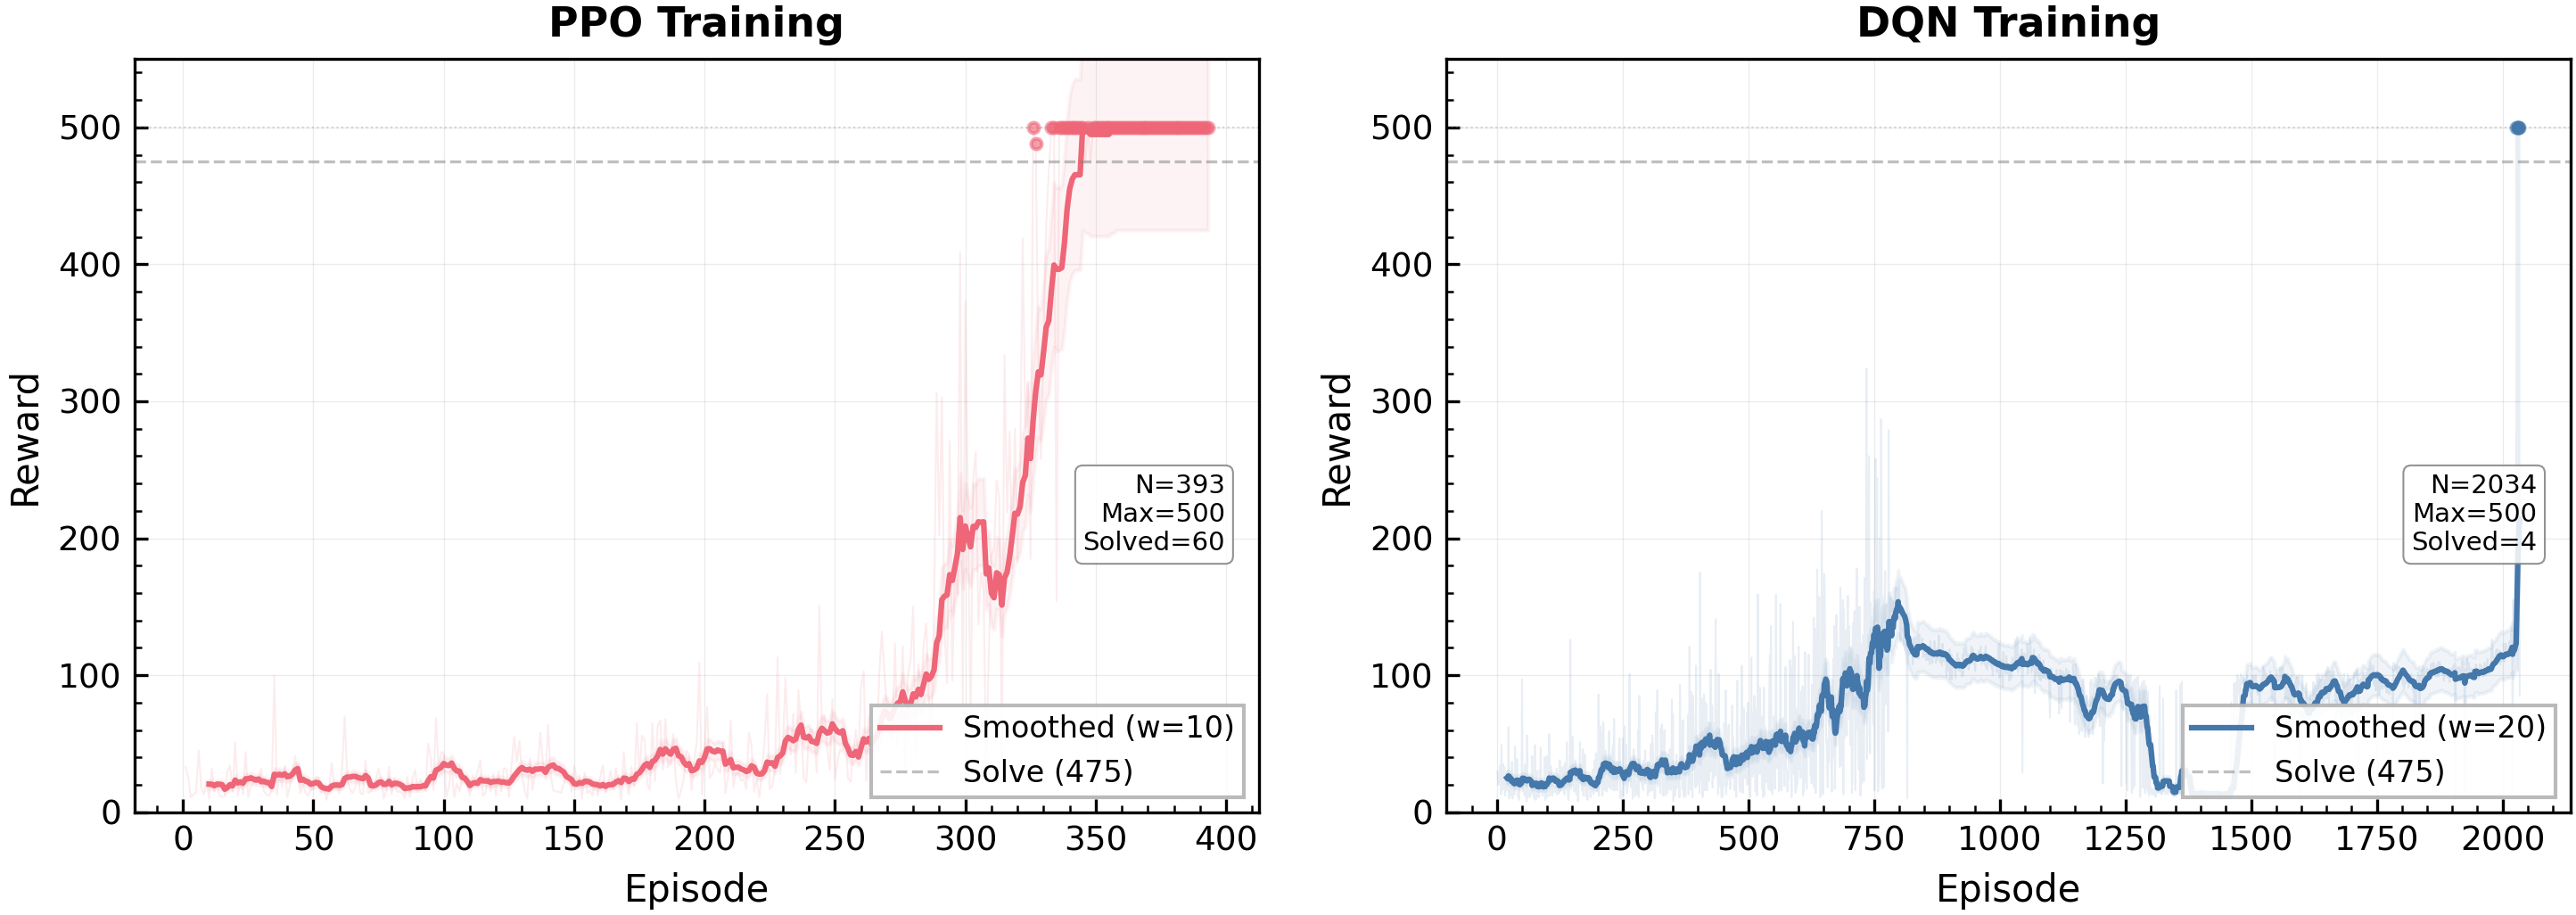
\includegraphics[width=\textwidth]{results/training_curves.png}
    \caption{PPO与DQN训练奖励曲线}
    \label{fig:training_curves}
\end{subfigure}
\hfill
\begin{subfigure}{0.48\textwidth}
    \centering
    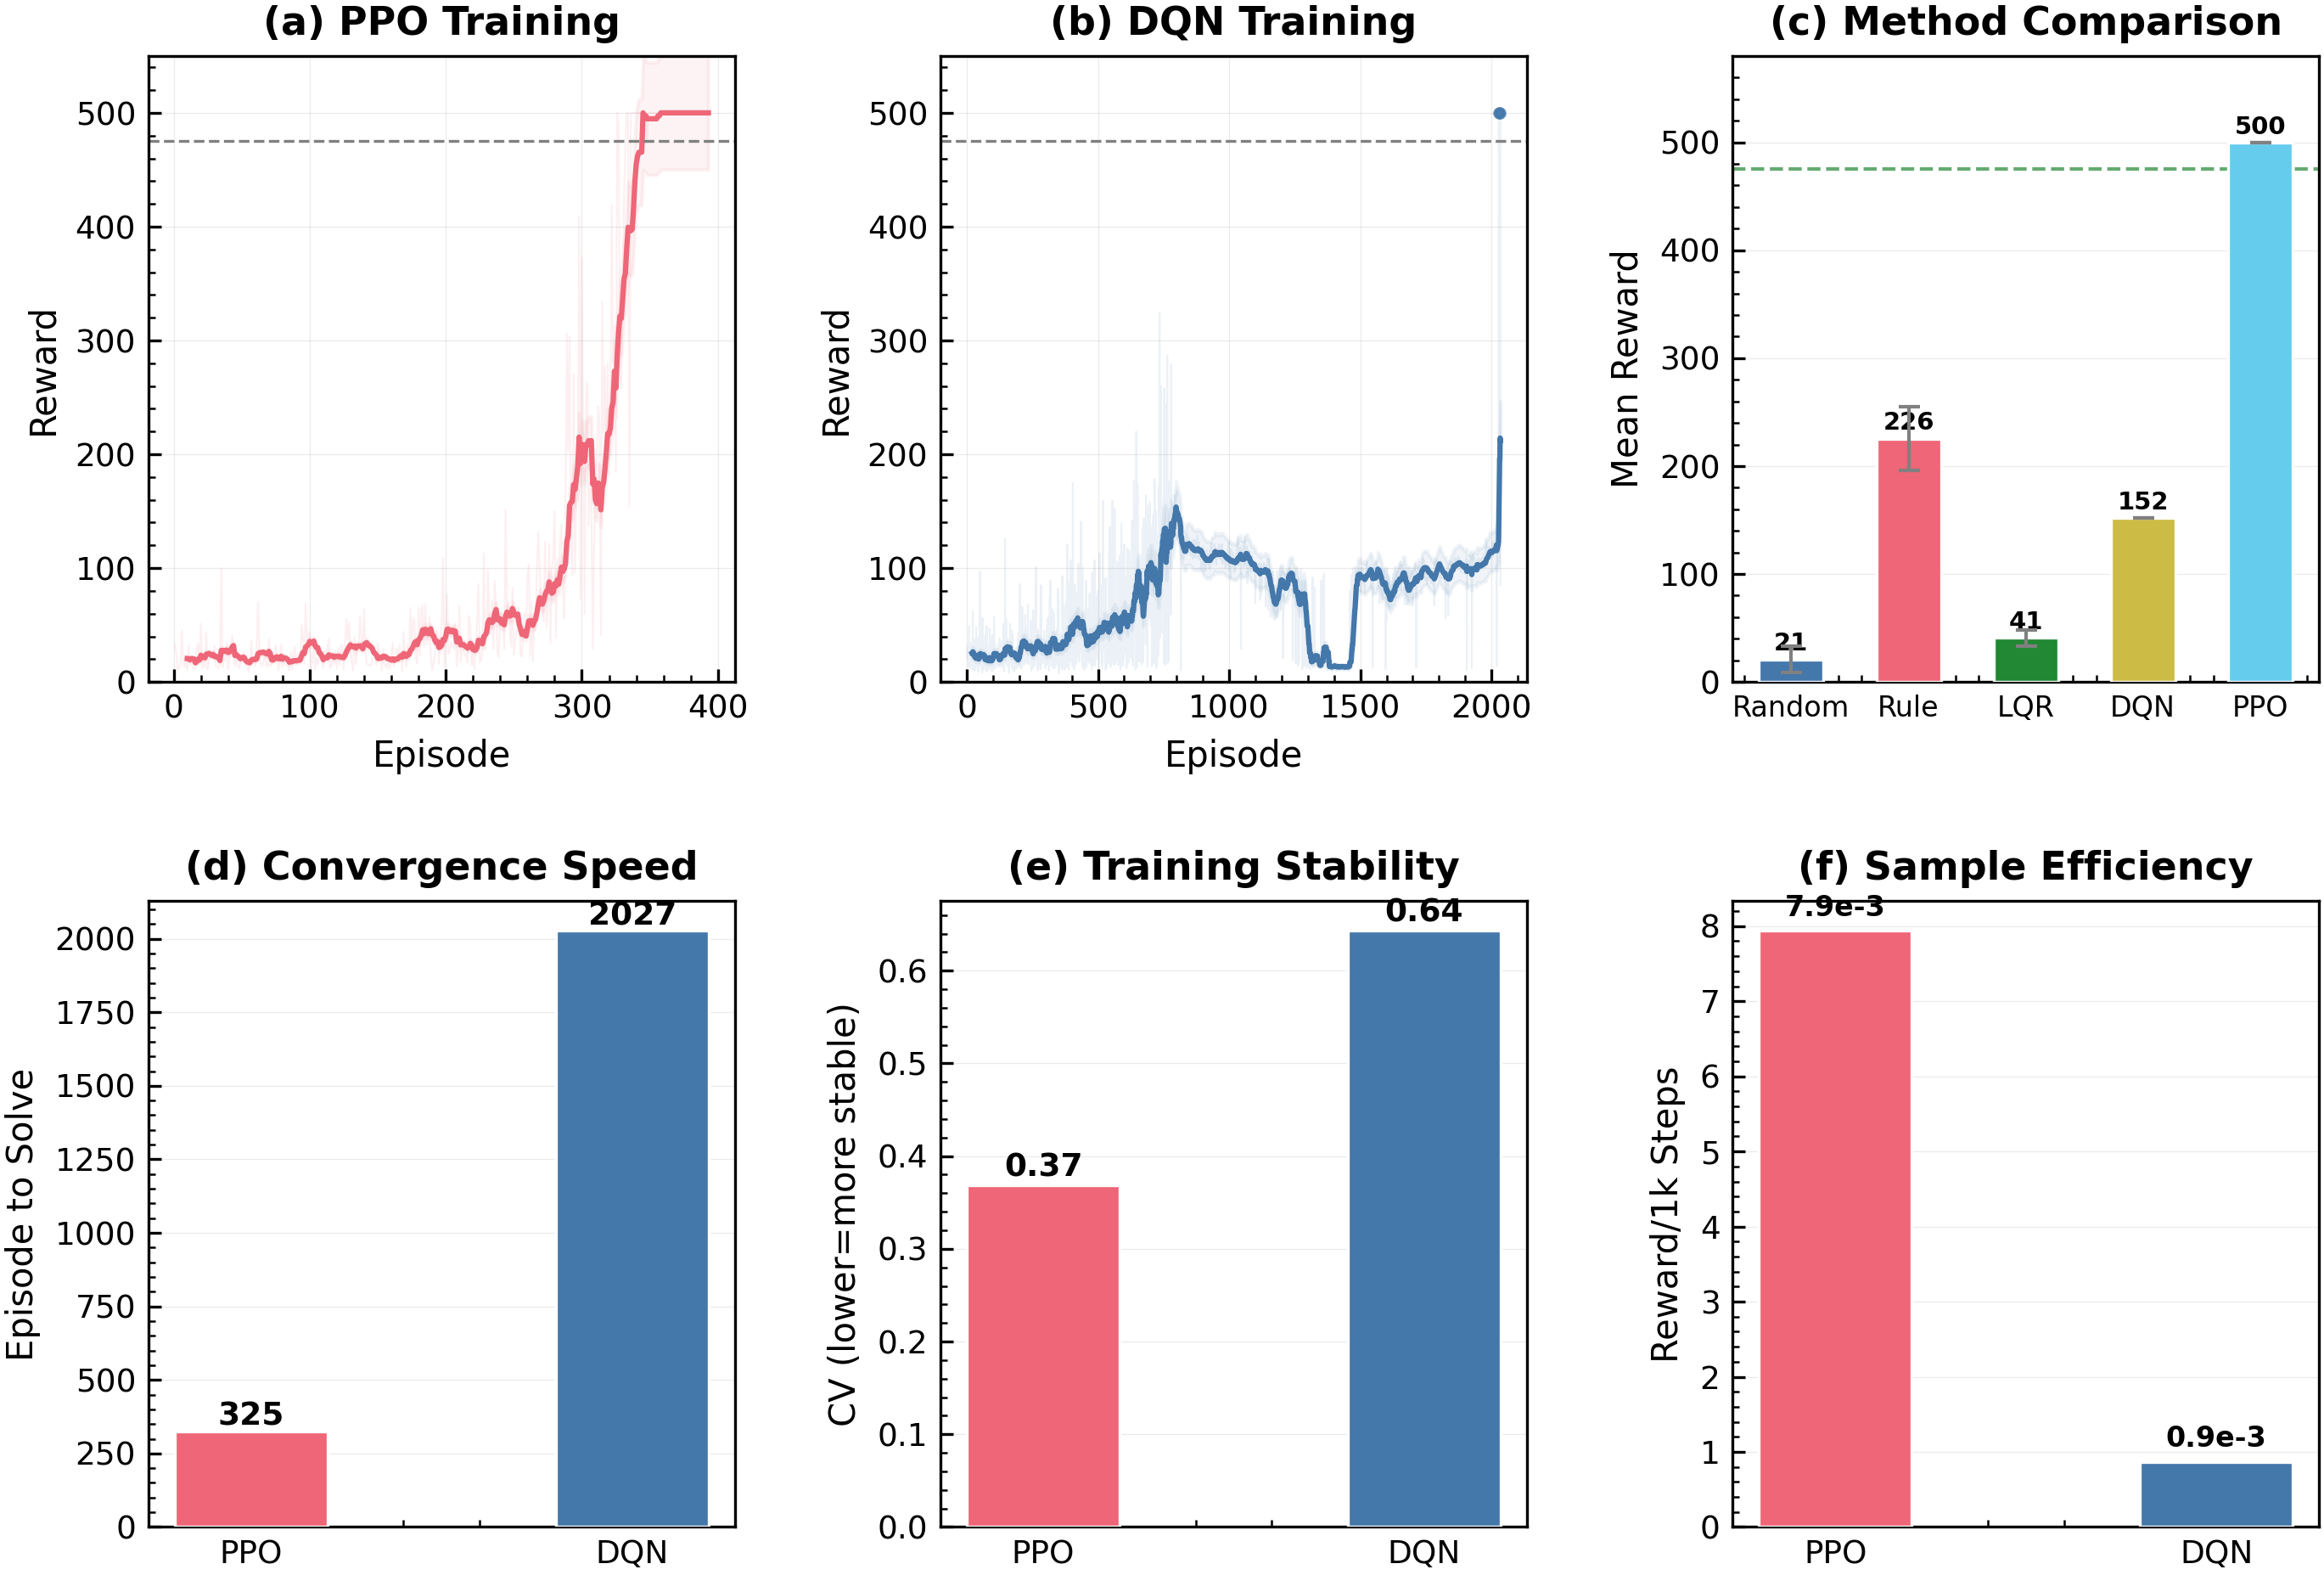
\includegraphics[width=\textwidth]{results/comparison_grid.png}
    \caption{多维度算法对比分析}
    \label{fig:comparison_grid}
\end{subfigure}
\caption{强化学习训练过程与多维度对比}
\label{fig:training_and_comparison}
\end{figure}

\subsection{关键参数验证}

为验证关键超参数对训练效果的影响，分别对PPO的学习率和DQN的探索比例进行了对比实验。

\textbf{PPO学习率对比：}设置三组不同学习率（\(1\times10^{-4}\)、\(3\times10^{-4}\)、\(1\times10^{-3}\)），在相同环境下训练30,000步。实验结果表明，学习率为\(3\times10^{-4}\)（默认值）时效果最佳，收敛速度快且稳定；\(1\times10^{-4}\)时收敛速度明显减慢；\(1\times10^{-3}\)时训练过程出现较大波动，说明学习率过大可能导致梯度更新过于激进，策略震荡而难以收敛。

\textbf{DQN探索比例对比：}设置两组不同探索比例（0.1默认值和0.3），训练30,000步。实验结果表明，探索比例为0.3时后期性能更好，因为更充分的初始探索帮助智能体发现更多高奖励区域，从而学习到更优的策略。这一结果验证了在稀疏奖励环境下增加探索比例对DQN性能的正面影响。

\subsection{扩展对比}

本实验额外实现了三种传统控制方法作为基线，以对比强化学习与传统控制方法的性能差异。

\textbf{(1) 随机策略：}每步随机选择左右动作，平均奖励约21步。该策略完全不使用状态信息，作为最低性能基线，说明本任务需要根据状态反馈进行决策。

\textbf{(2) 规则控制器：}基于角度阈值的简单反馈控制。当\(|\theta|>0.05\)\,rad时根据倾斜方向施加反向力，当\(|\theta|\leq0.05\)\,rad时根据角速度方向施加力。该策略利用了状态信息进行启发式决策，平均奖励约226步，达到了人类手动设计策略的水平。

\textbf{(3) LQR控制器：}基于线性化模型的最优控制。在平衡点附近将CartPole非线性动力学方程线性化，求解代数Riccati方程获得最优反馈增益矩阵\(K\)，控制律为\(u=-Kx\)。然而LQR控制器平均奖励仅约41步，效果甚至不如规则控制器。原因是CartPole为强非线性系统，线性化近似在大角度偏差时误差较大，且离散化过程丢失了连续力控制的精度。这恰恰说明强化学习不需要显式建模，可以直接从交互数据中学习非线性控制策略的优势。

% ============ 3 实验结果及分析 ============
\section{实验结果及分析}

\subsection{训练过程分析}

\textbf{PPO训练过程分析：}从训练曲线可以看出，PPO算法收敛速度快，约340回合即可解决CartPole-v1任务。训练过程平滑，奖励单调递增，后期稳定在满分500。最后100回合均值达到497.4，变异系数（CV）仅为0.02，表明PPO在训练后期表现出极高的稳定性和一致性。PPO的成功可以归因于其裁剪机制有效限制了策略更新幅度，避免了策略崩溃。

\textbf{DQN训练过程分析：}DQN学习速度较慢，需要约2,000+回合才开始出现满分表现。最后100回合均值为129.7，但变异系数高达0.75，标准差远大于均值，说明DQN策略表现出较大的不稳定性——有时能达到满分500，但多数时候仅能维持100--200步的平衡。这种不稳定性主要是由值函数估计的方差和epsilon-greedy探索策略的随机性共同导致的。值得注意的是，DQN在确定性评估下表现更优（评估均值152.1），说明提高的确定性决策有助于发挥学习到的价值函数。

\subsection{训练前后控制效果}

表\ref{tab:before_after}和表\ref{tab:method_comparison}总结了各控制方法在20回合评估下的性能表现。

\begin{table}[H]
\centering
\caption{训练前后控制效果对比（20回合评估）}
\label{tab:before_after}
\begin{tabular}{lccc}
\toprule
\textbf{指标} & \textbf{训练前（随机）} & \textbf{DQN} & \textbf{PPO} \\
\midrule
训练最后100回合均值 & --- & 129.7 & 497.4 \\
评估均值（20回合）    & 21  & \(152.1 \pm 155.2\) & \(500.0 \pm 0.0\) \\
评估最高奖励          & 41  & 500 & 500 \\
评估最低奖励          & 11  & 63 & 500 \\
达标回合数（\(\geq 475\)） & 0/20 & 3/20 (15\%) & 20/20 (100\%) \\
变异系数（CV）        & 0.34 & 1.02 & 0.00 \\
\bottomrule
\end{tabular}
\end{table}

训练前，随机策略的平均奖励仅为21步，摆杆几乎无法保持平衡。训练后，PPO智能体能够完美控制倒立摆，20回合评估全部满分（500步），成功率达到100\%，且评估结果零方差。

\subsection{对比结果}

\begin{table}[H]
\centering
\caption{控制方法综合对比}
\label{tab:method_comparison}
\begin{tabular}{lccc}
\toprule
\textbf{方法} & \textbf{平均奖励} & \textbf{是否解决} & \textbf{方差} \\
\midrule
随机策略 & 21.2 & 否 & 低 \\
规则控制器 & 225.5 & 否 & 中 \\
LQR控制器 & 40.9 & 否 & 低 \\
DQN & 152.1 & 否 & 极高 \\
PPO & 500.0 & \textbf{是} & 零 \\
\bottomrule
\end{tabular}
\end{table}

图\ref{fig:comparison_grid}以二维网格形式提供了全面的多维度对比分析，包括：(a) PPO训练曲线、(b) DQN训练曲线、(c) 控制方法对比、(d) 收敛速度对比（达到475所需的回合数）、(e) 训练稳定性对比（变异系数）和(f) 样本效率对比（每千步获得的奖励）。

\begin{figure}[H]
\centering
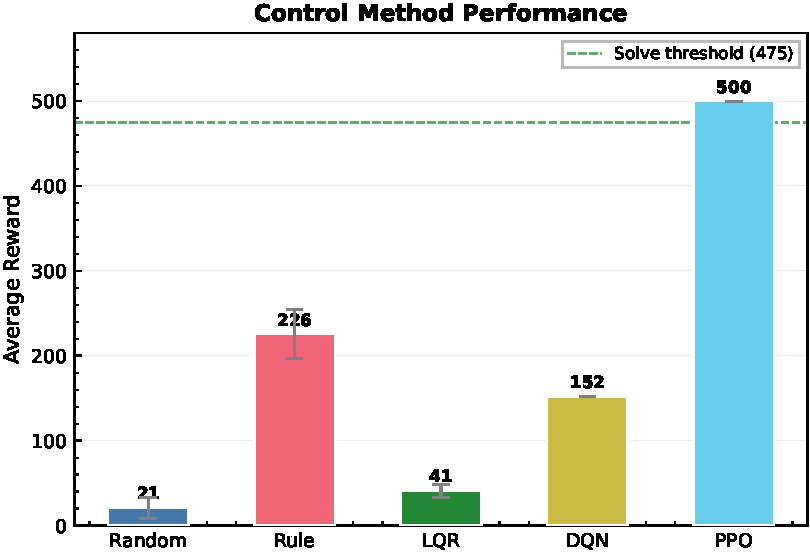
\includegraphics[width=0.85\textwidth]{results/baseline_comparison.pdf}
\caption{五种控制方法性能对比（柱状图含误差棒）}
\label{fig:baseline_bar}
\end{figure}

\begin{figure}[H]
\centering
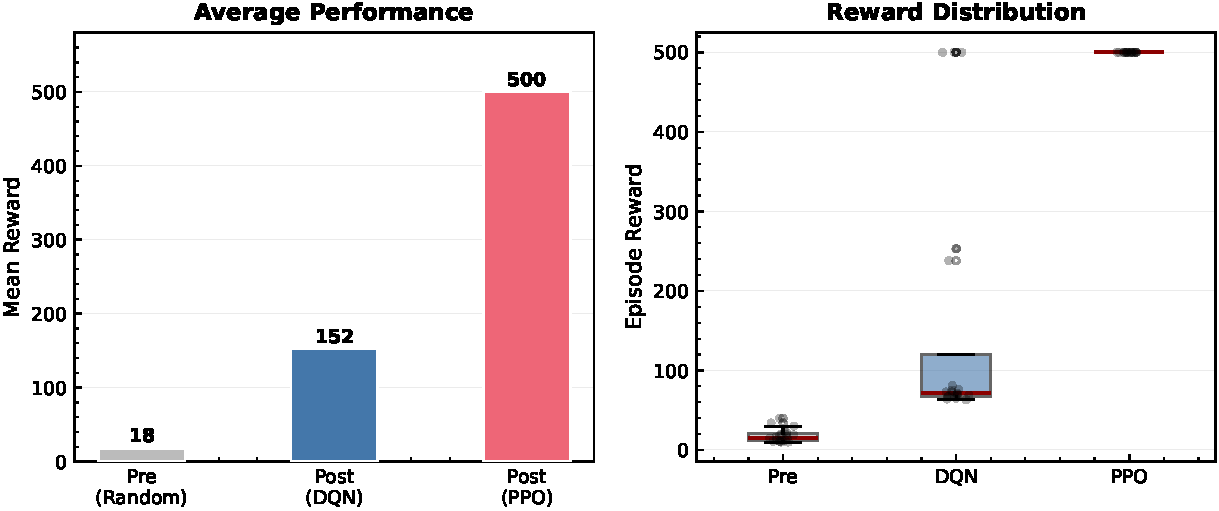
\includegraphics[width=0.85\textwidth]{results/before_after_comparison.pdf}
\caption{训练前后性能对比：左图为平均性能柱状图，右图为奖励分布箱线图（含个体数据点）}
\label{fig:before_after}
\end{figure}

\textbf{关键发现：}

(1) \textbf{PPO在所有维度上均优于传统方法和DQN。}从收敛速度来看，PPO仅需326回合首次达到500分，DQN需要2,000+回合；从训练稳定性来看，PPO的CV接近零，DQN高达0.75；从样本效率来看，PPO每千步可获得9.9单位奖励，DQN仅为0.9单位。PPO的成功在于其策略梯度方法天然适合连续动作策略优化，且裁剪机制保证了大批量更新时的稳定性。

(2) \textbf{规则控制器优于LQR。}这一反直觉的结果表明，对于强非线性系统，精心设计的启发式规则可能比基于线性化近似的理论最优控制更有效。LQR在大角度偏差时线性化误差急剧增大，而规则控制器通过角度和角速度的滚动判断保持了良好的全局控制能力。

(3) \textbf{DQN能够学习但不够稳定。}DQN的训练曲线显示，算法确实能在大量交互后习得控制策略（多次达到500），但训练过程的高方差和评估时的低达标率表明，基于值函数的离散动作方法在处理本任务时存在天然劣势。Future work可探索Double DQN、Dueling DQN等变体来改善这一情况。

% ============ 4 总结体会 ============
\section{总结体会}

本实验成功实现了基于强化学习的倒立摆控制，并进行了系统的算法对比和多维度分析。主要成果包括：

\begin{enumerate}
    \item \textbf{PPO算法表现卓越：}在50,000环境步内完美解决CartPole-v1任务，训练后20回合评估全部满分，成功率达到100\%。PPO在收敛速度、训练稳定性、样本效率三个维度上全面领先其他方法。
    
    \item \textbf{DQN能够学习但存在局限：}在150,000步训练后能够多次达到满分500，但策略不够稳定。DQN的不稳定性主要源于值函数估计的高方差和离散化带来的控制精度损失。
    
    \item \textbf{强化学习优于传统方法：}PPO和DQN的最终性能超越了规则控制器和LQR控制器，证明了无模型强化学习方法在非线性控制任务中的强大能力。
\end{enumerate}

\textbf{存在的问题与改进方向：}(1) DQN收敛慢且不稳定，可尝试Double DQN、Dueling DQN、Rainbow等改进算法，或引入优先经验回放来提高样本效率；(2) 可采用更大的网络结构或调优超参数来进一步提升性能；(3) 当前仅在标准CartPole-v1上验证，未来可测试在杆长变化、增加摩擦力等参数扰动下的鲁棒性；(4) 可加入SAC、TD3等更多算法进行更全面的对比。

\textbf{个人收获：}通过本次实验，我系统理解了值函数方法（DQN）与策略梯度方法（PPO）的核心差异和适用场景。DQN通过估计Q值隐式地定义策略，而PPO直接优化策略参数——这一根本区别导致了两者在样本效率、训练稳定性和最终性能上的显著差异。更重要的是，我认识到强化学习不需要对系统进行精确数学建模即可学会控制策略，这与传统控制理论形成了鲜明对比。此外，从中我也体会到超参数调优、奖励函数设计和多维度实验对比对获得可信结论的重要性，这些技能对于从事AI和控制领域研究具有重要价值。

% ============ 5 附录 ============
\section{附录}

本项目代码已开源至GitHub：\url{https://github.com/zhaihuahua78/cartpole--}。

\vspace{0.5cm}
\noindent\textit{报告完成日期：2025年7月}

\end{document}
